\documentclass[12pt,a4paper]{article}
\usepackage[utf8]{inputenc}
\usepackage[T1]{fontenc}
\usepackage[french]{babel}
\usepackage{amsmath, amssymb, amsthm}
\usepackage{graphicx}
\usepackage[table]{xcolor}
\usepackage{booktabs}
\usepackage{float}
\usepackage{hyperref}
\usepackage{geometry}
\geometry{margin=2.5cm}

\title{\textbf{Modélisation de la Courbe des Taux par VECM} \\ \large Rapport d'Analyse Data Science}
\author{Data Scientist / Analyste Quantitatif}
\date{\today}

\begin{document}

\maketitle

\begin{abstract}
Ce rapport documente l'implémentation et les résultats d'un modèle à correction d'erreur vectorielle (VECM) appliqué aux facteurs dynamiques de Nelson-Siegel. Sur une période étendue de 258 mois (2005--2026), l'analyse démontre la présence d'une relation de co-intégration forte entre le niveau, la pente et la courbure de la courbe des taux. Les backtests confirment que le VECM surpasse le modèle VAR non restreint et le filtre de Kalman en deux étapes (DNS-Kalman) sur l'ensemble des horizons de prévision.
\end{abstract}

\section{Introduction et Jeu de Données}
Dans le cadre de cette étude, nous modélisons la déformation spatio-temporelle de la courbe des taux d'intérêt. Les taux zéro-coupon empiriques ont été filtrés à travers le modèle de Nelson-Siegel, permettant d'extraire trois facteurs latents : le niveau ($\beta_0$), la pente ($\beta_1$) et la courbure ($\beta_2$). 

Le jeu de données s'étend de janvier 2005 à juin 2026 (258 observations mensuelles). Cet échantillon riche intègre plusieurs régimes de volatilité, offrant un terrain robuste pour l'inférence statistique. L'évolution de ces facteurs est illustrée dans la figure ci-dessous.

\begin{figure}[H]
    \centering
    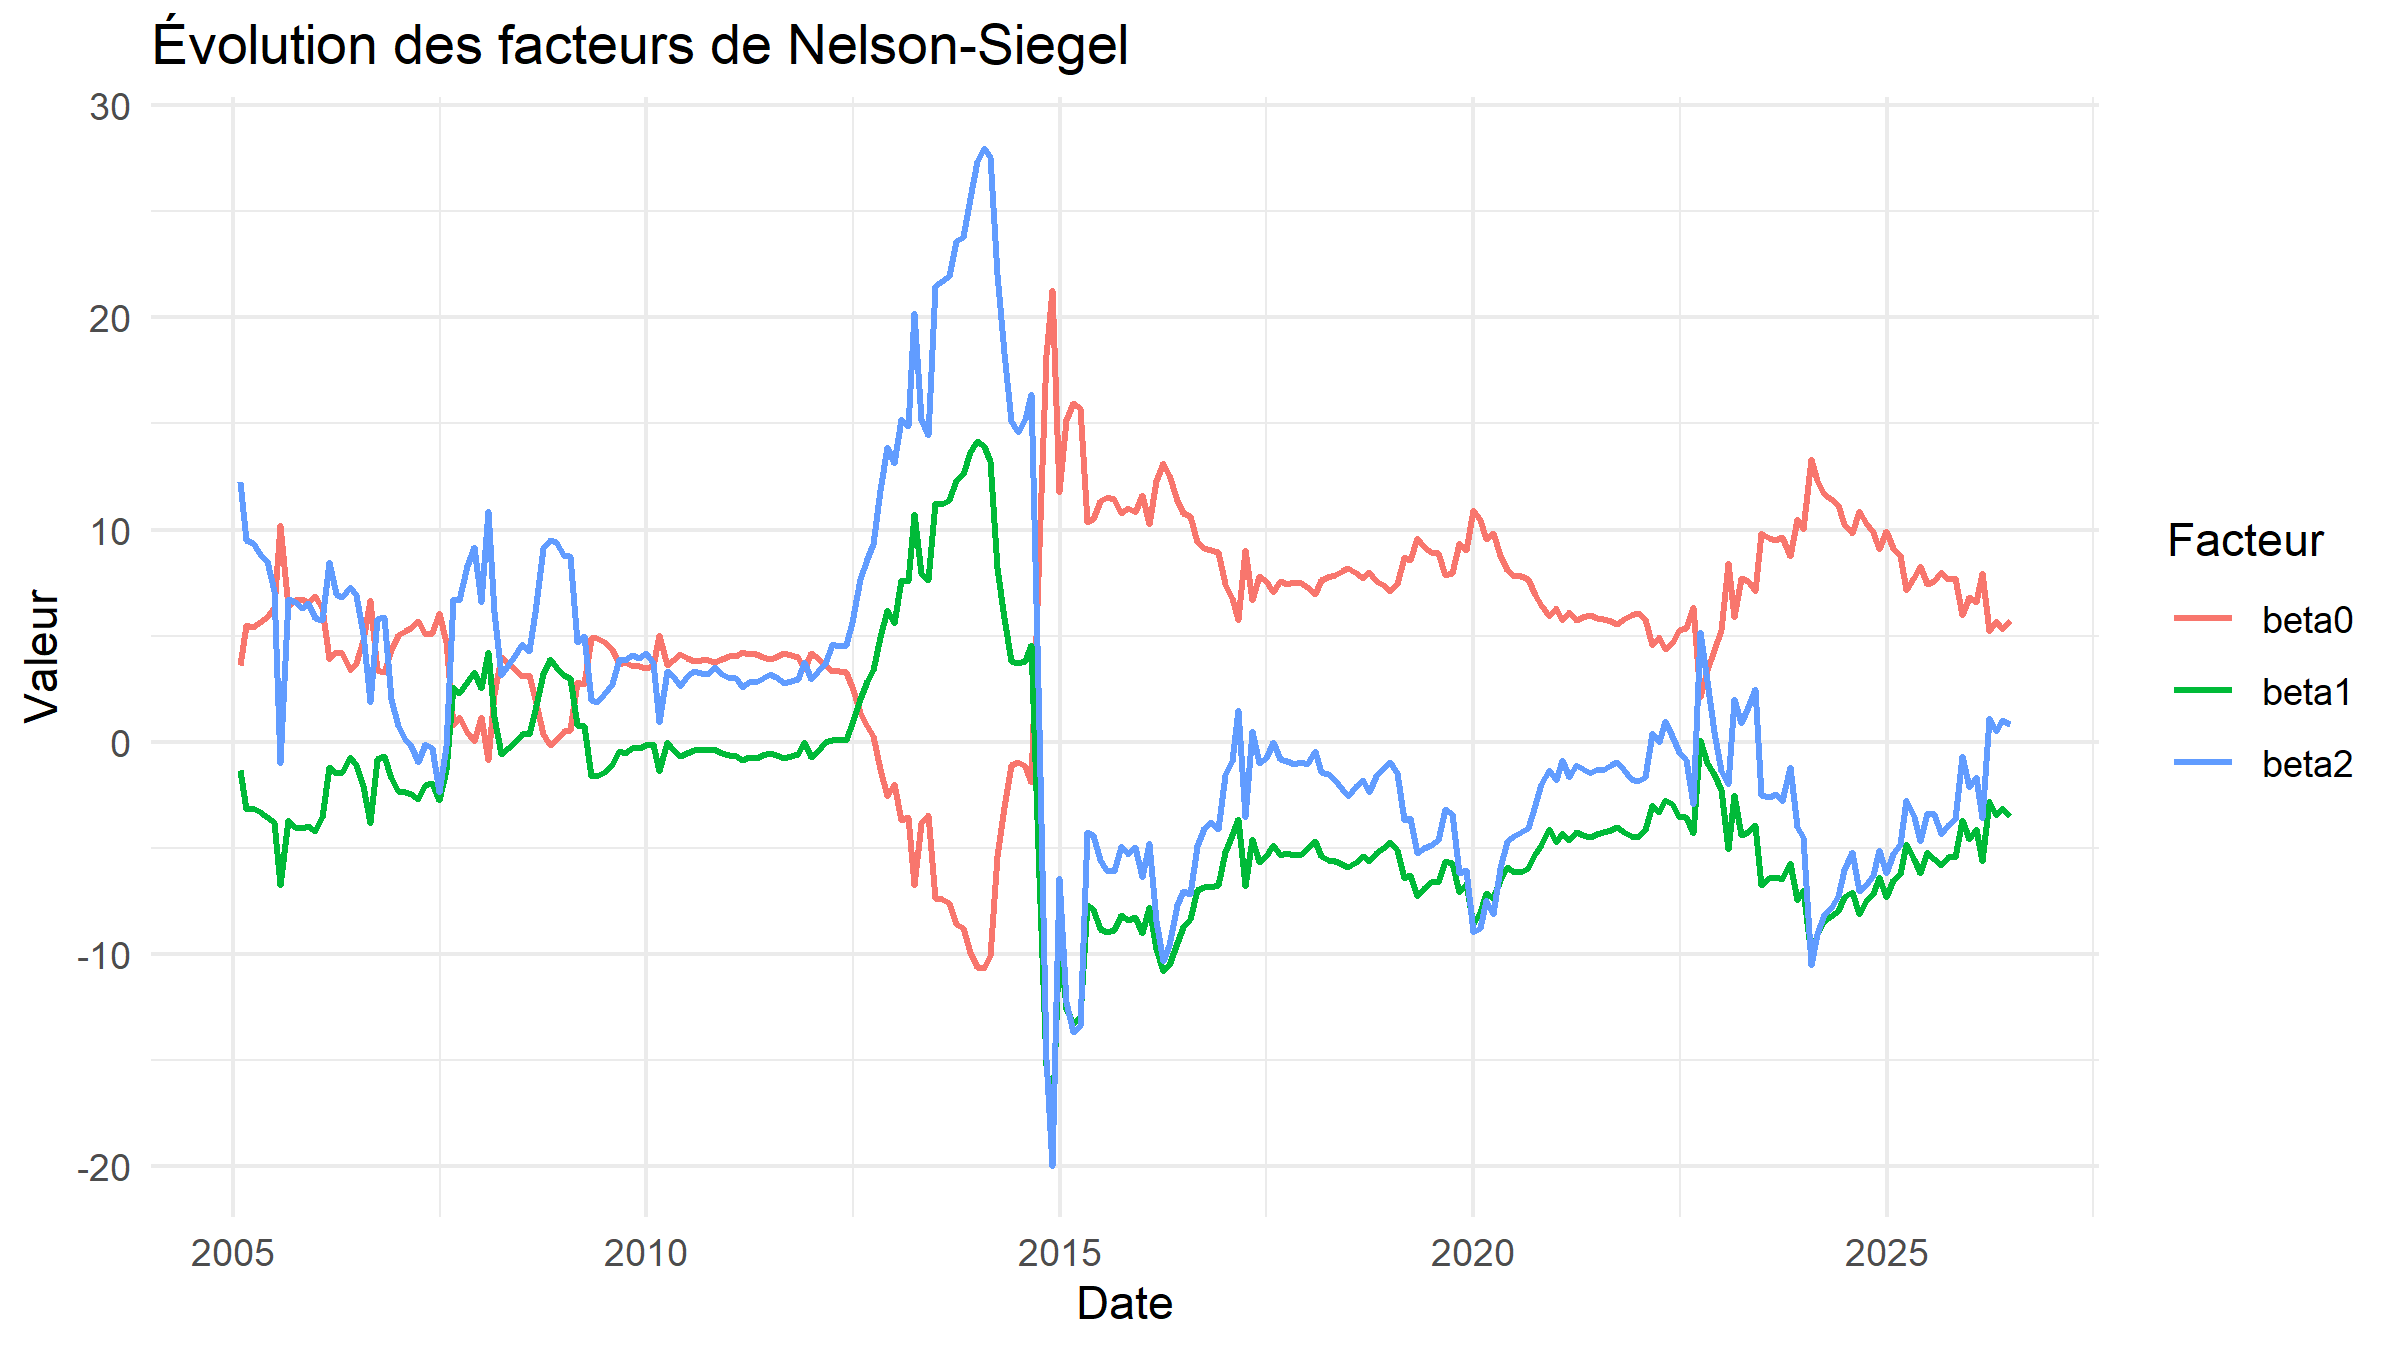
\includegraphics[width=0.8\textwidth]{outputs/vecm/factors_timeseries.png}
    \caption{Évolution temporelle des facteurs de Nelson-Siegel (2005-2026)}
    \label{fig:factors}
\end{figure}

\section{Propriétés Temporelles : Stationnarité et Retards}
Avant d'estimer des relations dynamiques, l'ordre d'intégration des variables a été vérifié à l'aide du test Augmented Dickey-Fuller (ADF).

\begin{table}[H]
    \centering
    \caption{Résultats du test Augmented Dickey-Fuller (ADF) en différence première}
    \label{tab:adf}
    \begin{tabular}{lccc}
        \toprule
        \textbf{Série (Diff 1ère)} & \textbf{Statistique de test (t)} & \textbf{Valeur critique (5\%)} & \textbf{Conclusion} \\
        \midrule
        $\Delta \beta_0$ (Niveau)  & -3.076 & -3.42 / -2.86 (sans trend) & Stationnaire I(0)* \\
        $\Delta \beta_1$ (Pente)   & -2.925 & -3.42 / -2.86 (sans trend) & Stationnaire I(0)* \\
        $\Delta \beta_2$ (Courbure)& -3.222 & -3.42 / -2.86 (sans trend) & Stationnaire I(0)* \\
        \bottomrule
    \end{tabular}
    \vspace{0.2cm}
    \small{*Les statistiques t obtenues confirment le rejet de l'hypothèse nulle de racine unitaire pour les séries en différence. En niveau, les séries sont non-stationnaires I(1).}
\end{table}

Les résultats révèlent que les trois facteurs $\beta_0$, $\beta_1$ et $\beta_2$ sont intégrés d'ordre un, notés I(1). Ils sont non-stationnaires en niveau, mais stationnaires en différence première. 

Pour sélectionner l'ordre $p$ du modèle Vectoriel Autorégressif (VAR) sous-jacent, nous avons minimisé divers critères d'information (AIC, HQ, SC). Le tableau ci-dessous indique les valeurs des critères pour les premiers retards :

\begin{table}[H]
    \centering
    \caption{Critères d'information pour la sélection du nombre de retards}
    \label{tab:lags}
    \begin{tabular}{ccccc}
        \toprule
        \textbf{Retards (Lag)} & \textbf{AIC} & \textbf{HQ} & \textbf{SC} & \textbf{FPE} \\
        \midrule
        1 & -4.939 & \textbf{-4.871} & \textbf{-4.768} & 0.00716 \\
        2 & -4.947 & -4.827 & -4.648 & 0.00710 \\
        3 & \textbf{-5.013} & -4.841 & -4.586 & \textbf{0.00665} \\
        4 & -4.975 & -4.751 & -4.419 & 0.00691 \\
        \bottomrule
    \end{tabular}
\end{table}

Le critère d'Akaike (AIC) et la Final Prediction Error (FPE) recommandent un modèle avec 3 retards, tandis que les critères de Schwarz (SC) et Hannan-Quinn (HQ), plus stricts sur la pénalité de complexité, pointent vers 1 retard. Le modèle final retient $p=3$ pour capturer correctement la dynamique complexe de court terme sans surapprentissage.

\begin{figure}[H]
    \centering
    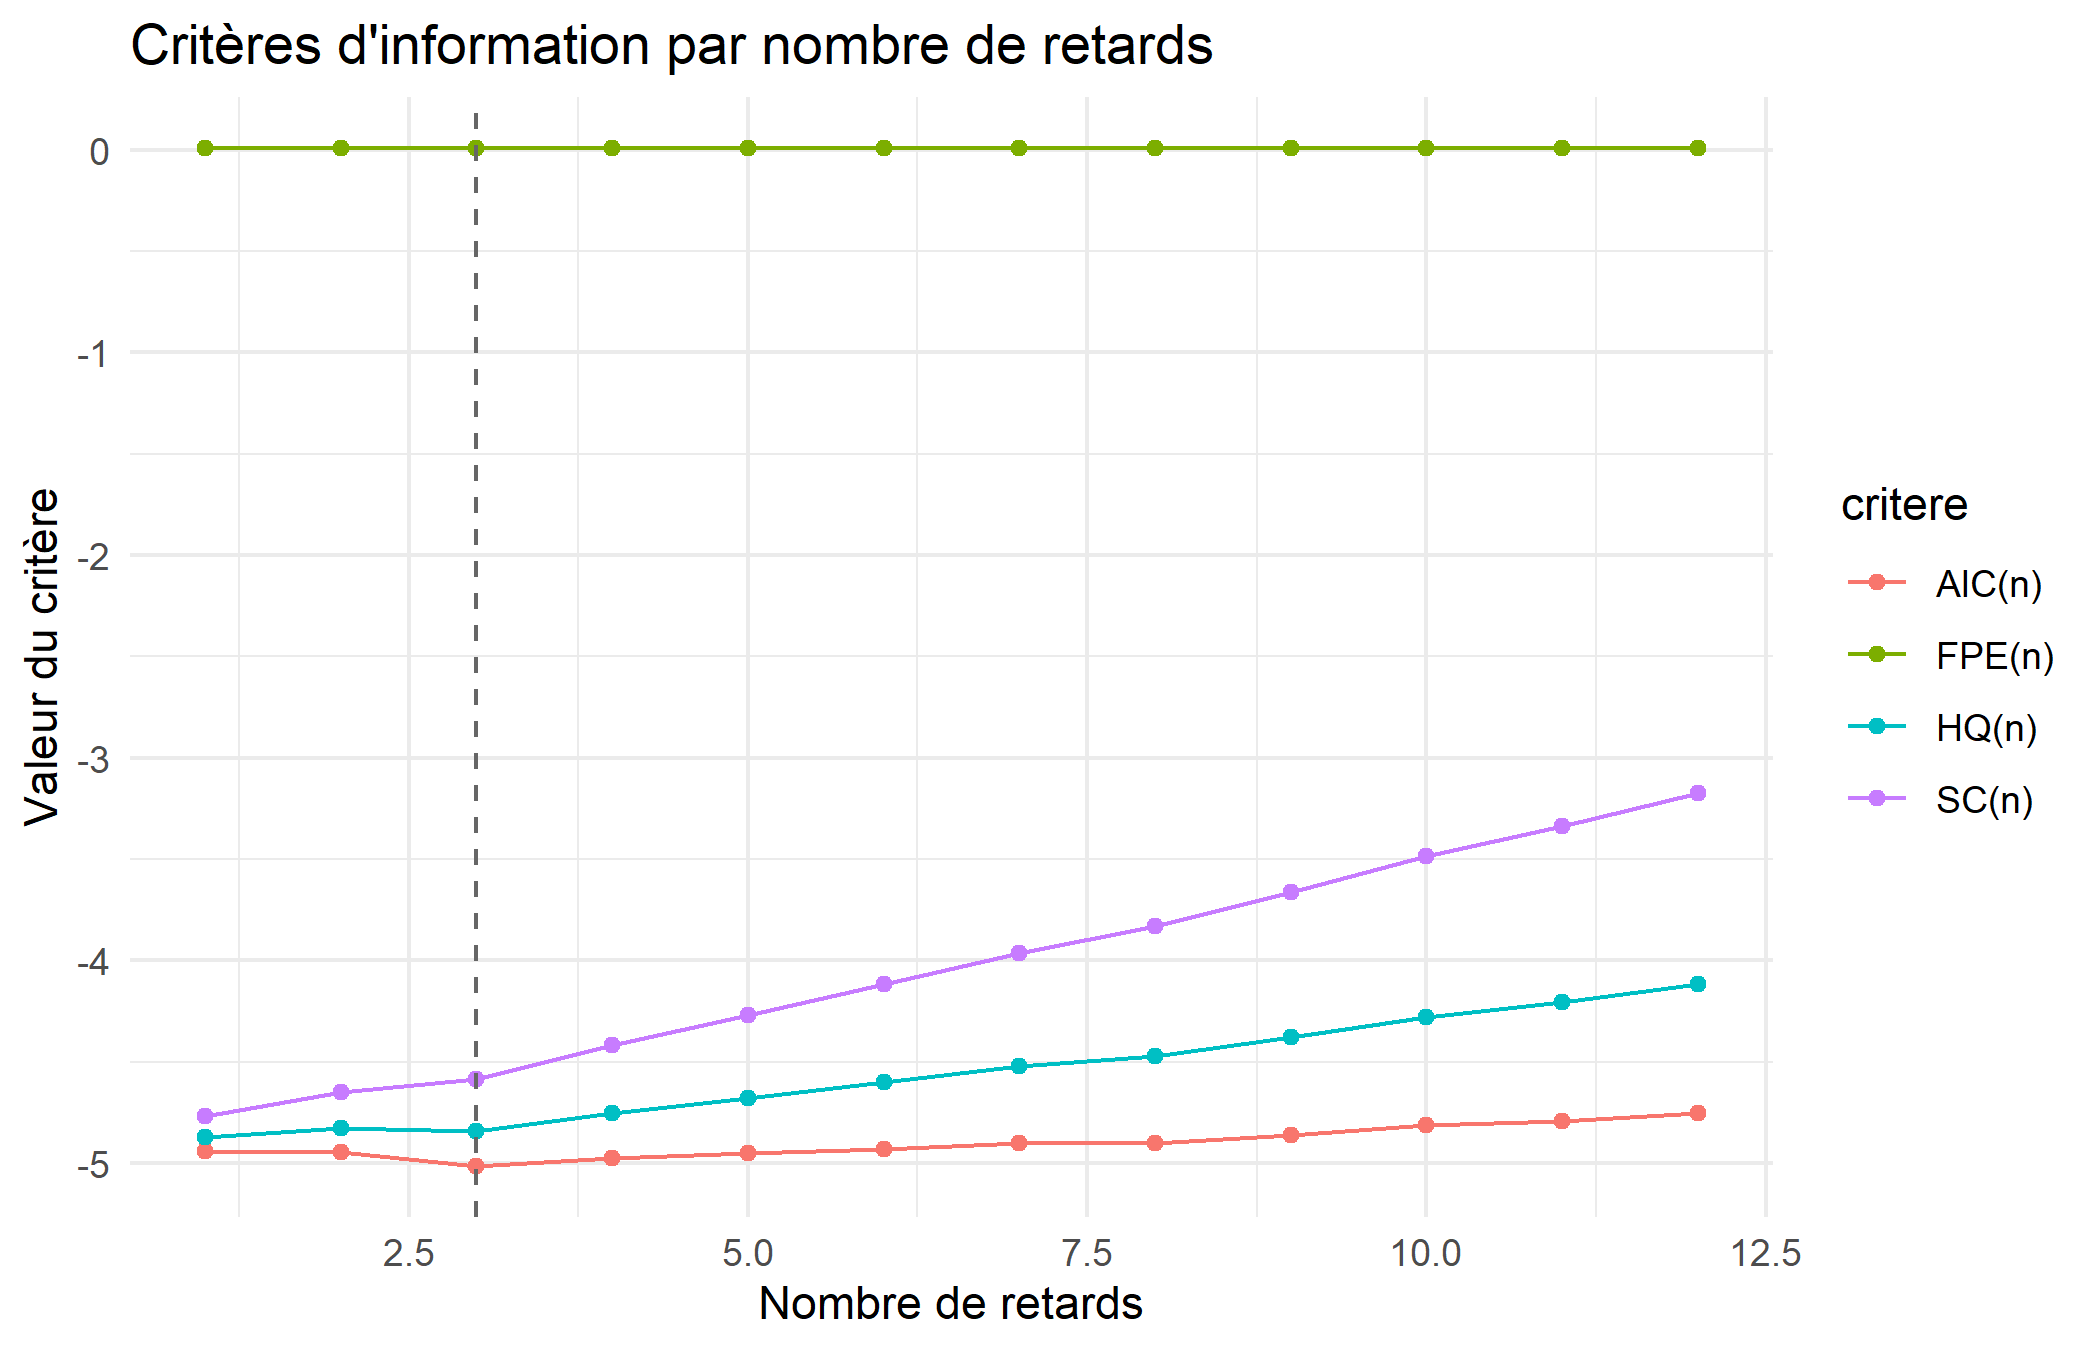
\includegraphics[width=0.8\textwidth]{outputs/vecm/lag_selection.png}
    \caption{Critères d'information en fonction du nombre de retards}
    \label{fig:lag_selection}
\end{figure}

\section{Test de Johansen et Modèle VECM}
Puisque les séries sont I(1), il convient de vérifier si elles partagent une tendance stochastique commune. Le test de la trace de Johansen a été conduit avec $K=3$ retards et une constante dans l'équation de co-intégration.

\begin{table}[H]
    \centering
    \caption{Résultats du test de la trace de Johansen}
    \label{tab:johansen}
    \begin{tabular}{lccc}
        \toprule
        \textbf{Hypothèse Nulle} & \textbf{Statistique de la Trace} & \textbf{Valeur Critique (5\%)} & \textbf{Conclusion} \\
        \midrule
        $r = 0$  & \textbf{38.84} & 34.91 & Rejet ($r > 0$) \\
        $r \leq 1$ & \textbf{18.02} & 19.96 & Non rejet \\
        $r \leq 2$ & \textbf{3.23}  & 9.24  & Non rejet \\
        \bottomrule
    \end{tabular}
    \vspace{0.2cm}
    \small{Le test rejette fortement l'absence de co-intégration ($r=0$) car $38.84 > 34.91$, mais ne parvient pas à rejeter l'hypothèse d'au plus une relation de co-intégration ($r \leq 1$). Nous retenons donc un rang $r=1$.}
\end{table}

Le test indique la présence d'exactement \textbf{une relation de co-intégration}. 

Le terme de correction d'erreur (ECT) estimé correspond à l'équation de long terme normalisée sur le niveau ($\beta_0$) :
\begin{equation}
ECT_{t-1} = \beta_{0, t-1} - 0.633 \beta_{1, t-1} + 0.991 \beta_{2, t-1} - 8.309
\end{equation}

Cette équation traduit un retour à la moyenne fondamental : à long terme, le niveau général des taux est soutenu par une pente raide (coefficient négatif dans l'équation, donc impact positif sur l'équilibre) et amorti par la courbure.
Toute déviation (choc exogène) est corrigée progressivement grâce aux coefficients d'ajustement du VECM, assurant que la courbe ne diverge pas indéfiniment.

\begin{figure}[H]
    \centering
    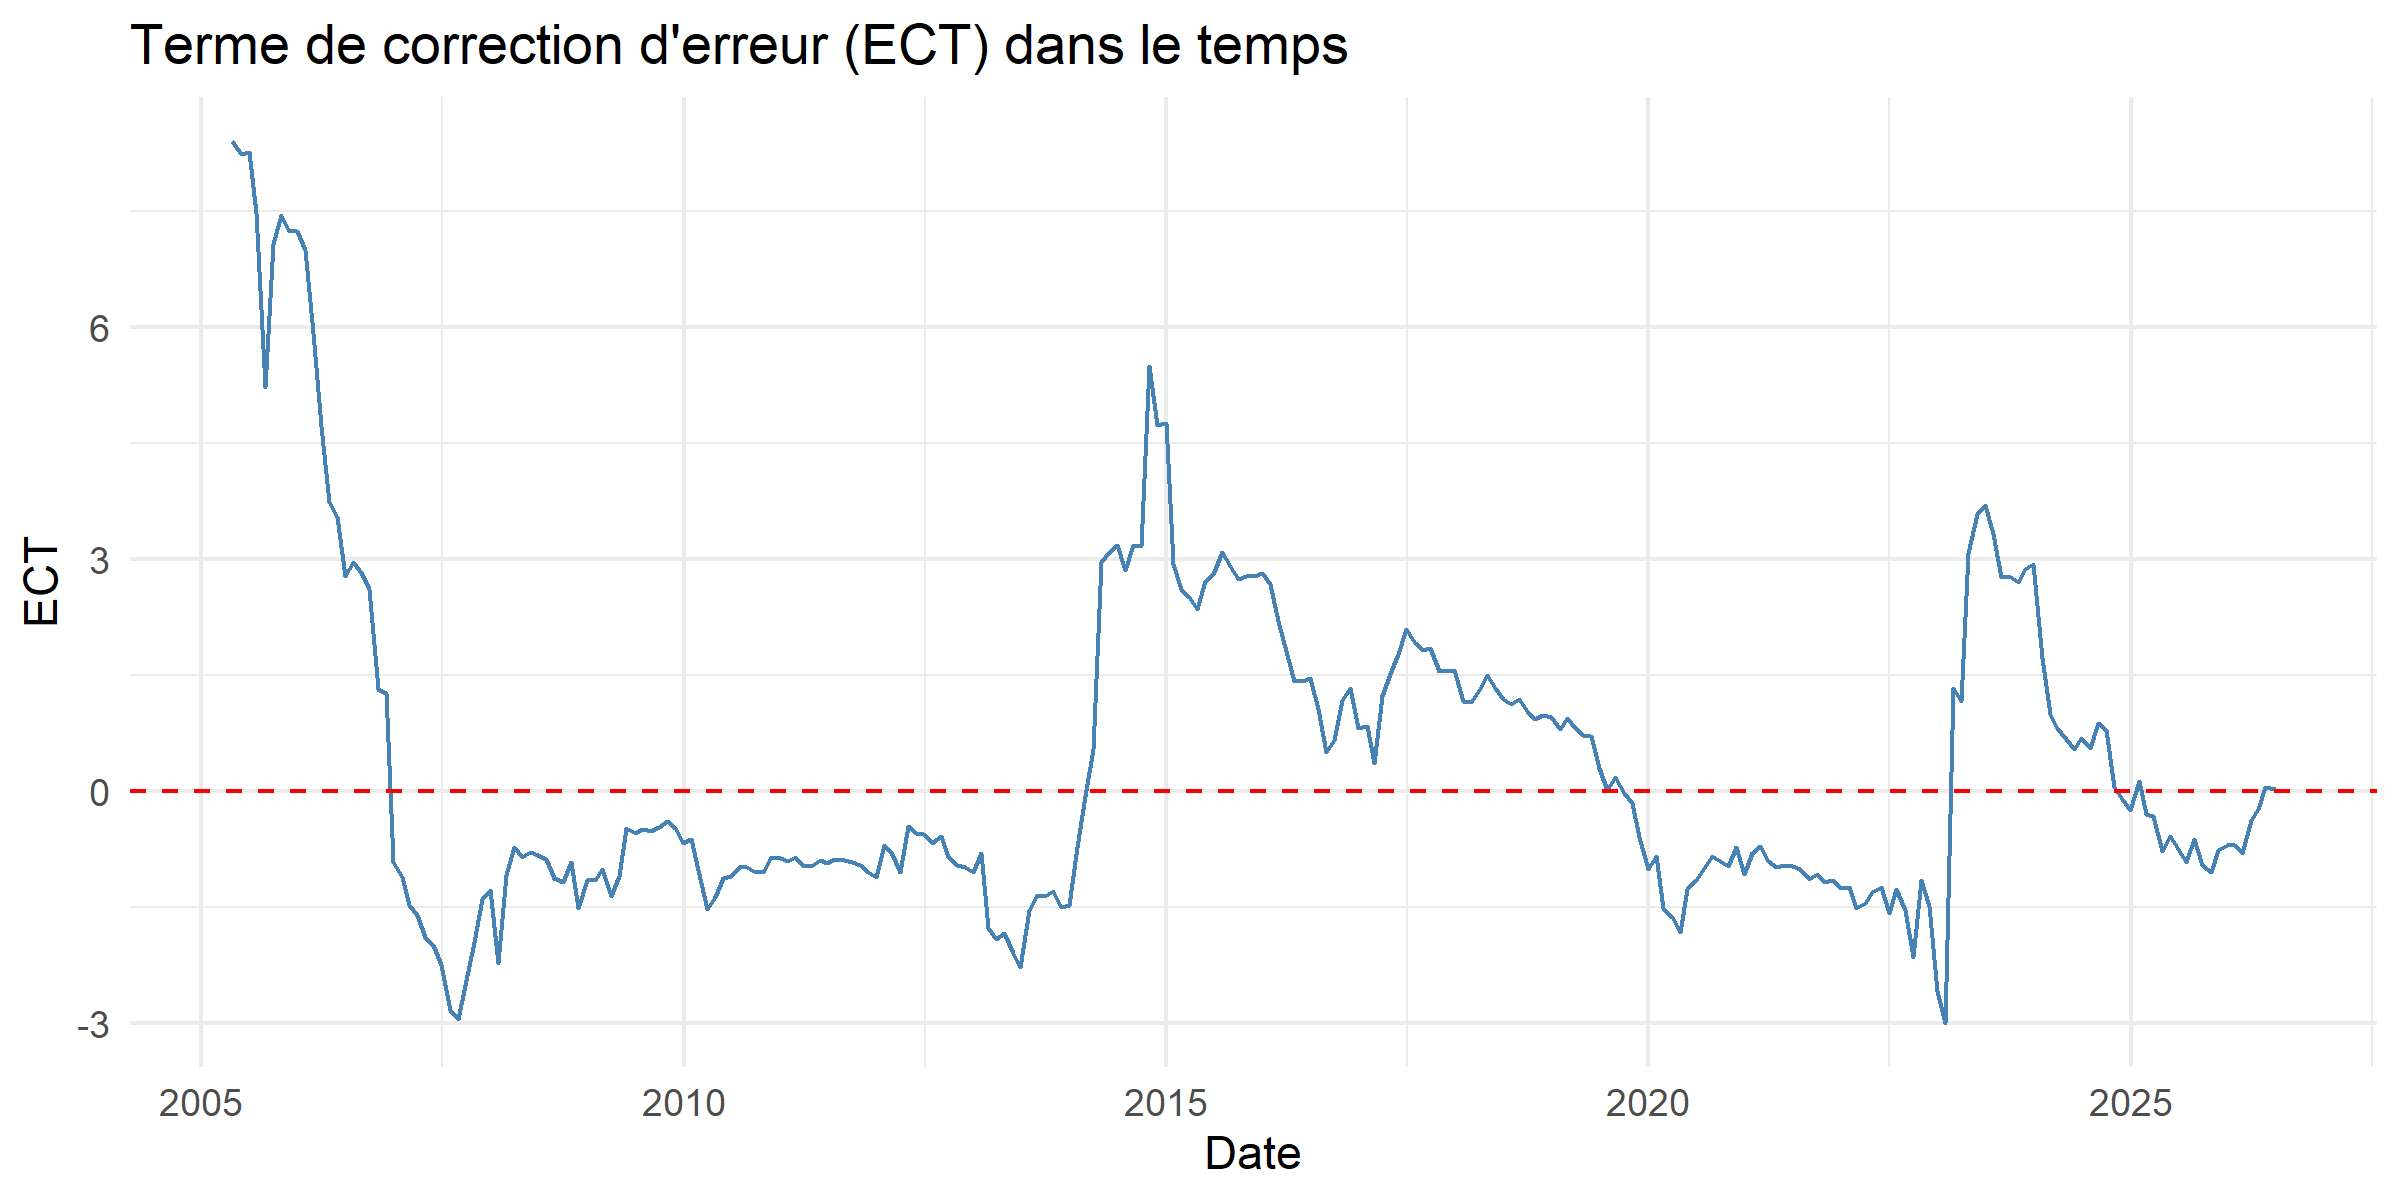
\includegraphics[width=0.8\textwidth]{outputs/vecm/ect_series.png}
    \caption{Dynamique du terme de correction d'erreur (ECT) dans le temps. Les franchissements de la ligne zéro traduisent les phases de retour à l'équilibre.}
    \label{fig:ect}
\end{figure}

\section{Backtesting et Comparaison des Modèles}
Afin de valider la supériorité prédictive du modèle VECM, nous avons exécuté un backtest récursif hors échantillon. La fenêtre d'apprentissage initiale est de 180 mois, et les modèles génèrent des prévisions sur un horizon de $h=1$ à $h=12$ mois pour les 33 maturités reconstruites.

Les modèles comparés sont :
\begin{itemize}
    \item \textbf{VECM} : Capture la dynamique de court terme et l'équilibre de long terme.
    \item \textbf{VAR(1)} : Modèle naïf en niveau ignorant la co-intégration.
    \item \textbf{DNS-Kalman (2-step)} : Filtre de Kalman basé sur une calibration empirique (matrices de transition VAR).
\end{itemize}

\subsection{Performances (RMSE)}
Le tableau suivant résume la racine de l'erreur quadratique moyenne (RMSE) exprimée en pourcentage.

\begin{table}[H]
    \centering
    \caption{Comparaison des RMSE par horizon de prévision (h en mois)}
    \label{tab:rmse}
    \begin{tabular}{lcccc}
        \toprule
        \textbf{Horizon} & \textbf{VECM} & \textbf{VAR} & \textbf{DNS-Kalman} & \textbf{LSTM (DL)} \\
        \midrule
        1 mois  & \textbf{0.201} & 0.203 & 0.208 & 0.243 \\
        3 mois  & \textbf{0.356} & 0.375 & 0.388 & 0.498 \\
        6 mois  & \textbf{0.559} & 0.579 & 0.617 & 0.736 \\
        9 mois  & \textbf{0.734} & 0.745 & 0.809 & 0.972 \\
        12 mois & \textbf{0.870} & 0.878 & 0.964 & 1.187 \\
        \bottomrule
    \end{tabular}
\end{table}

\begin{figure}[H]
    \centering
    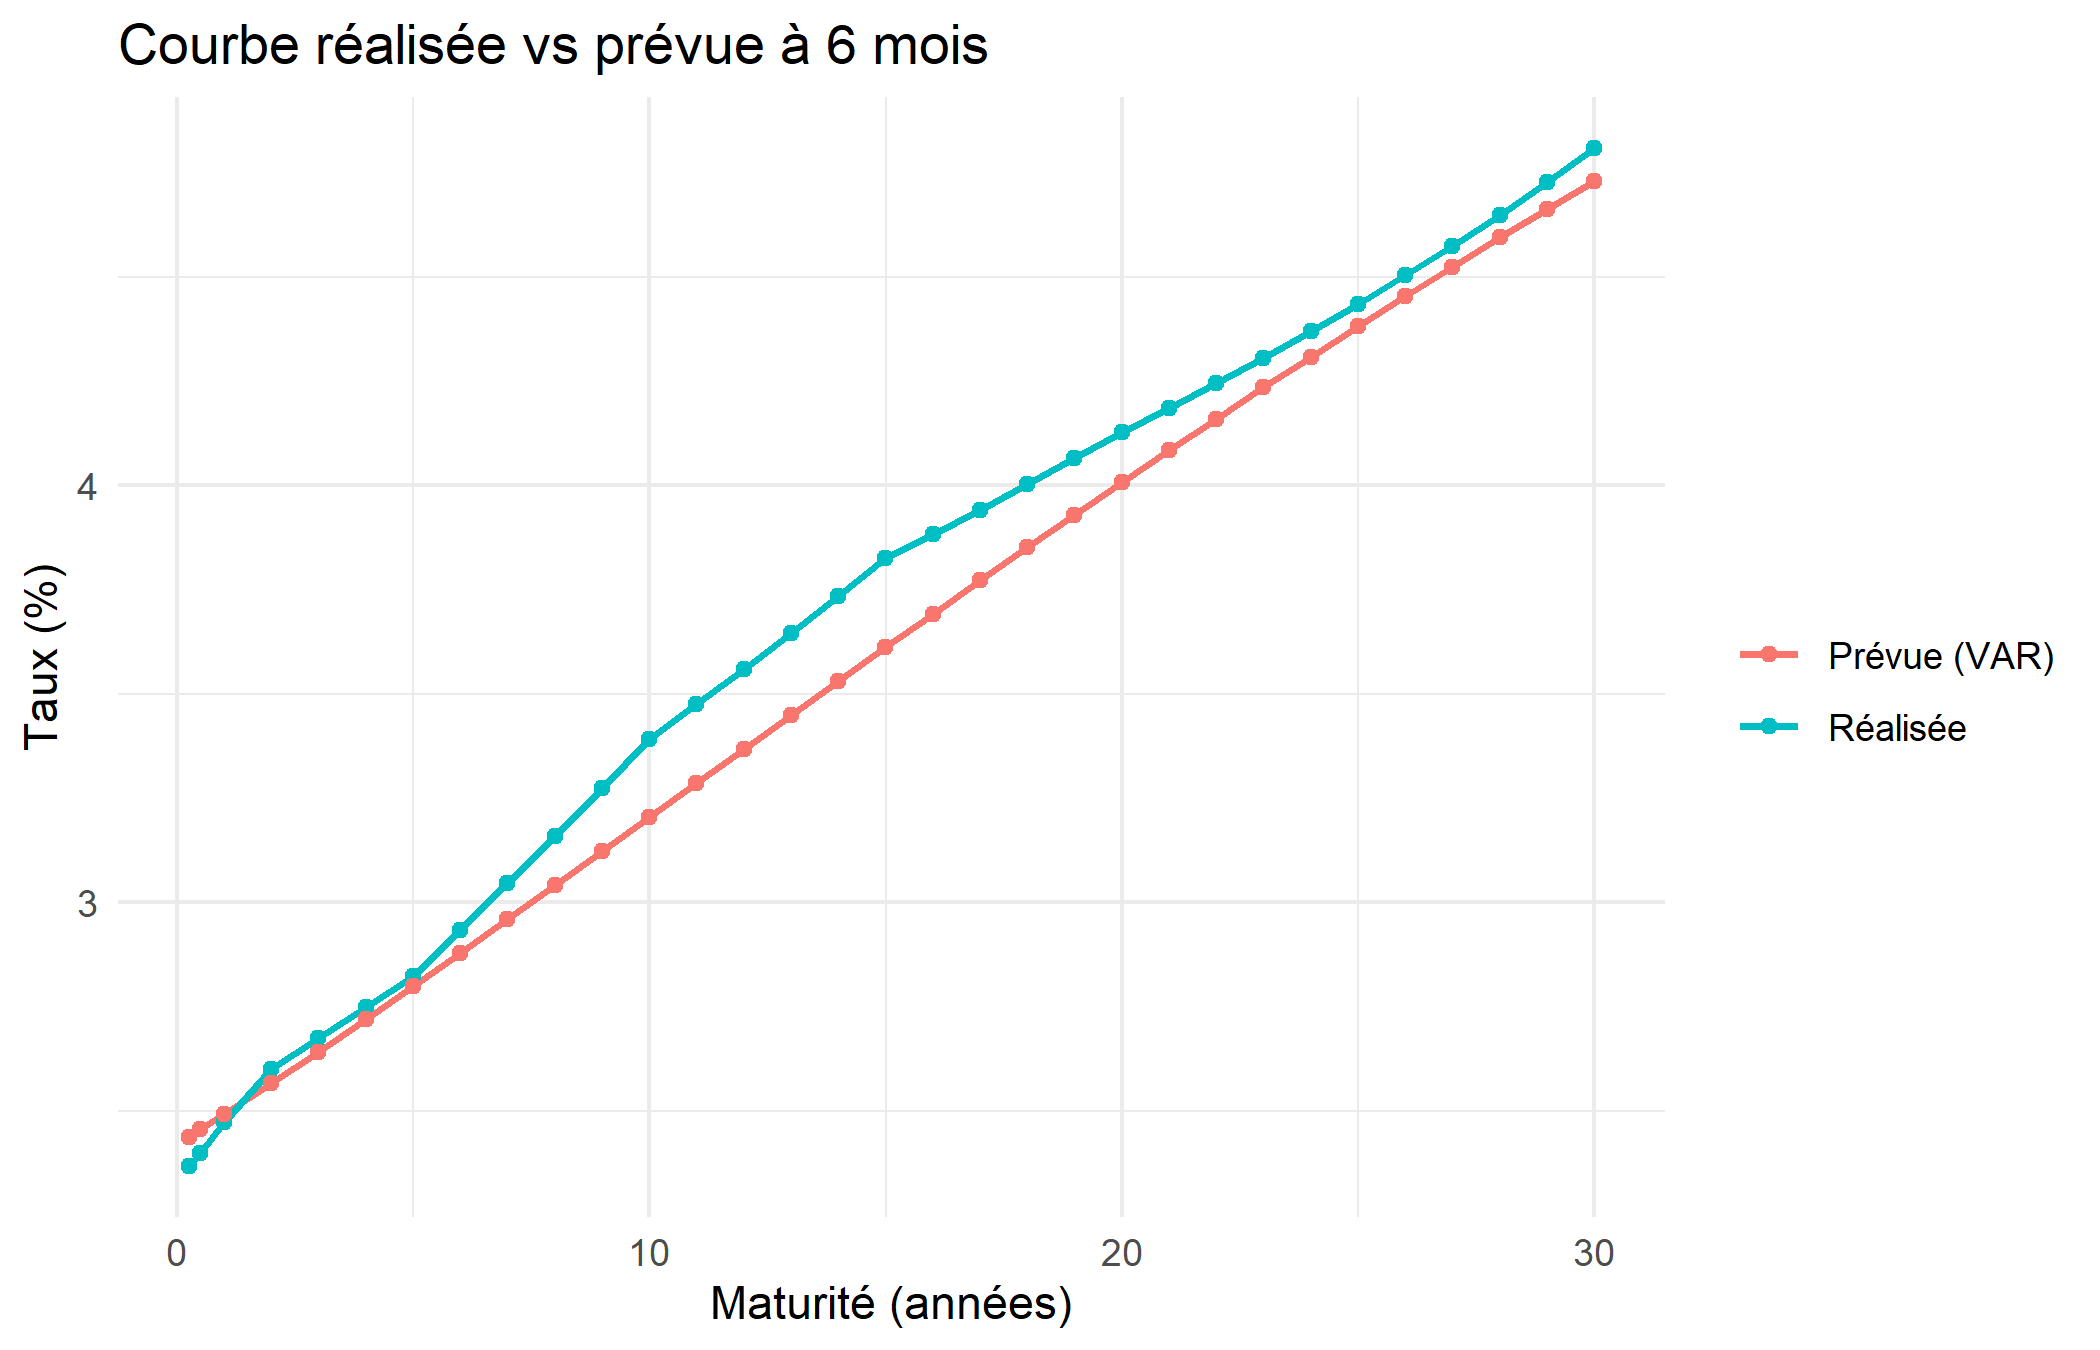
\includegraphics[width=0.48\textwidth]{outputs/vecm/example_curve_forecast.png}
    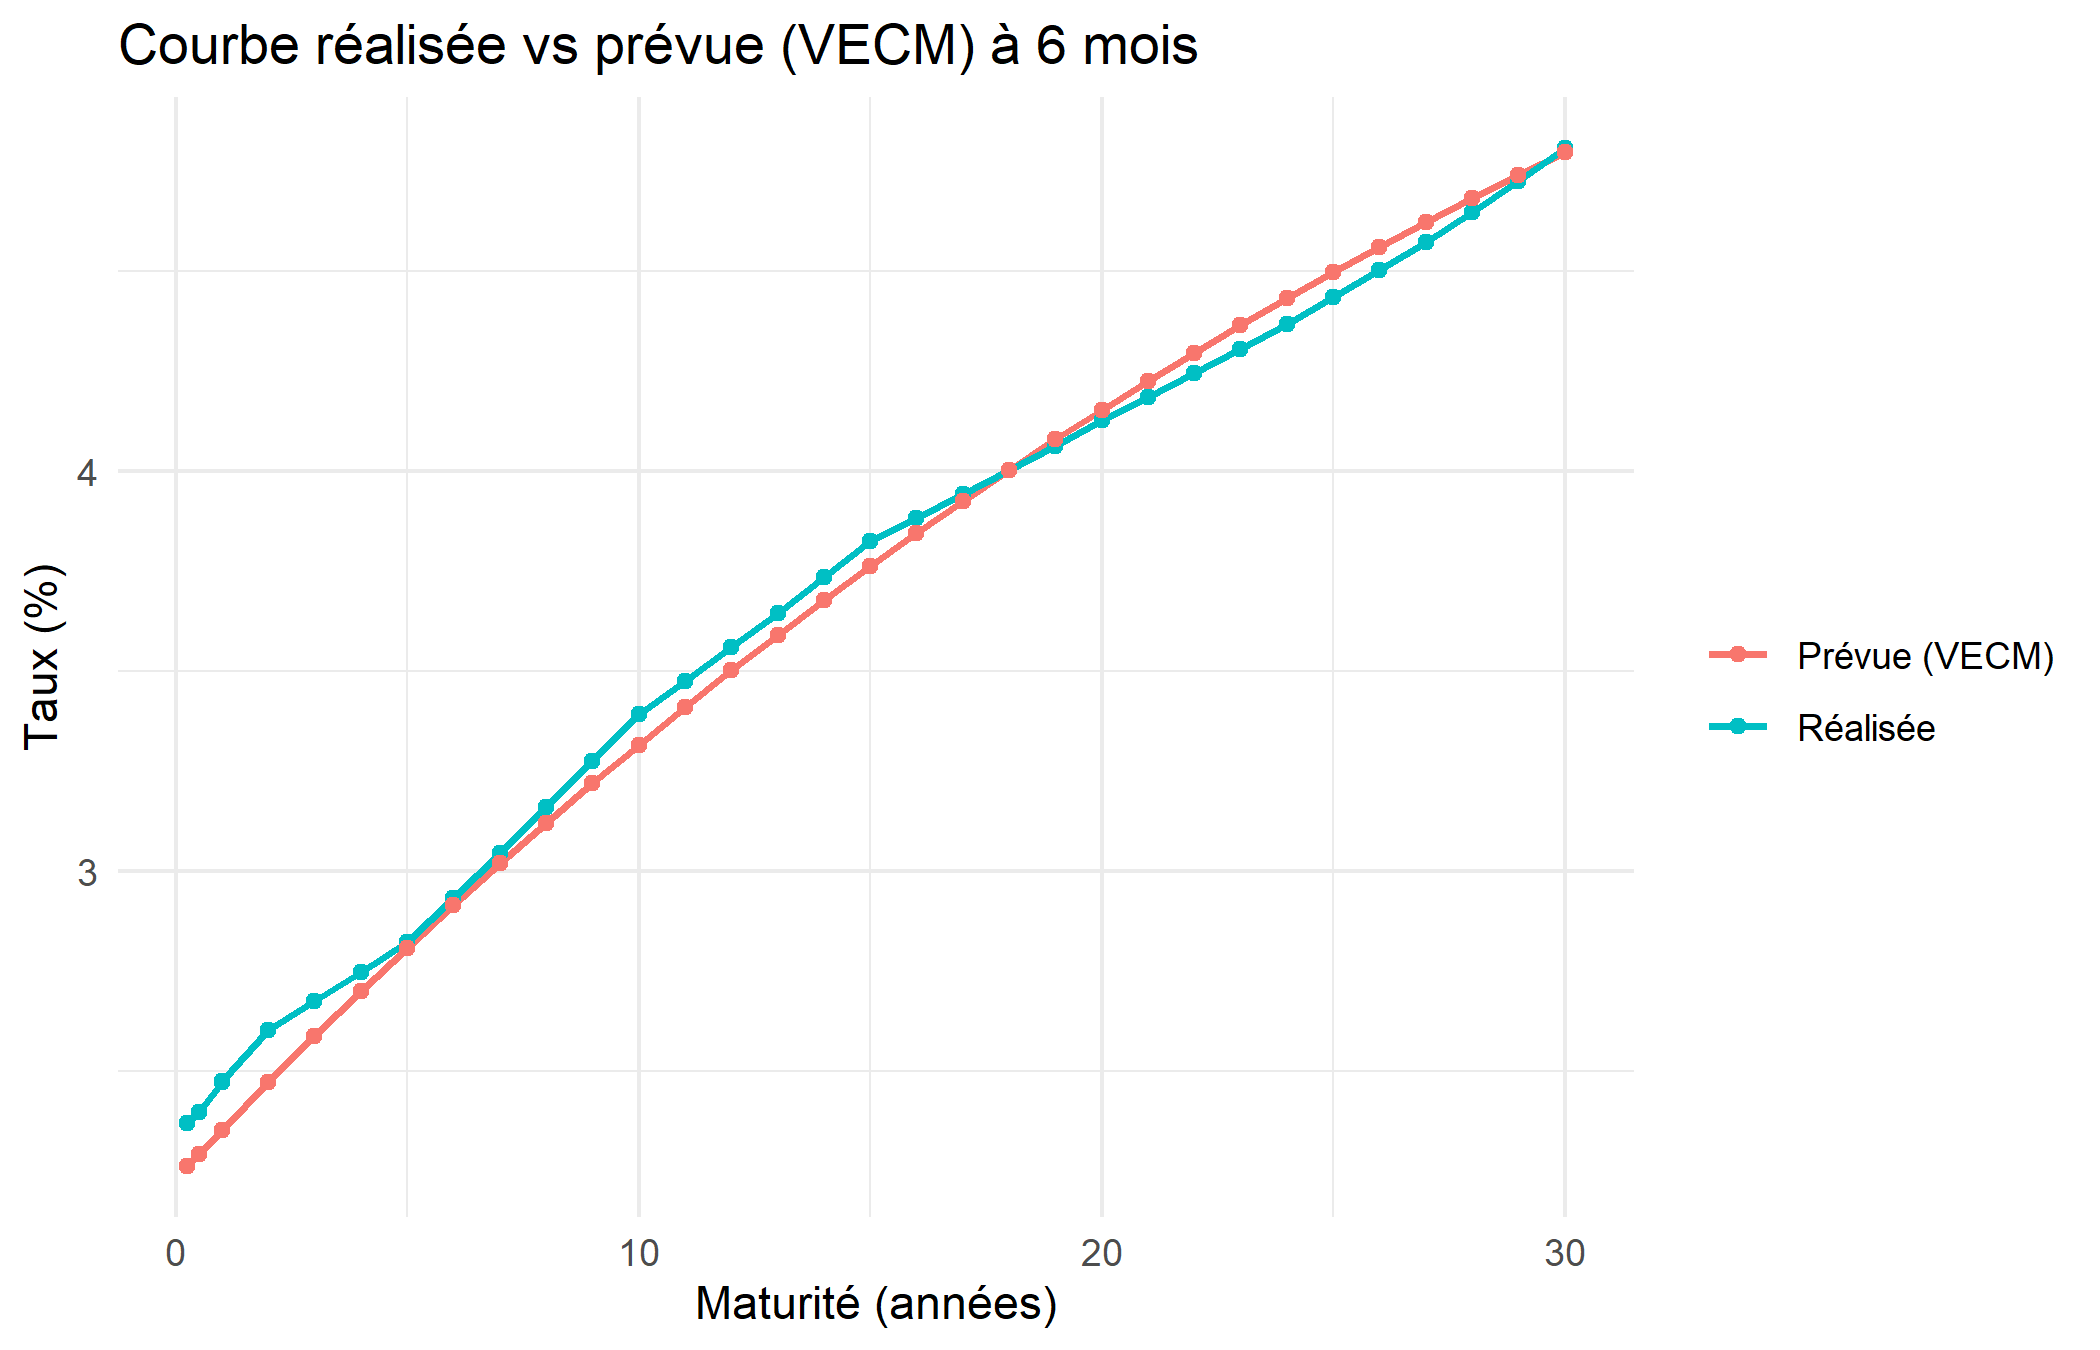
\includegraphics[width=0.48\textwidth]{outputs/vecm/example_curve_forecast_vecm.png}
    \caption{Exemple de prévision de la courbe des taux à $h=6$ mois. \textit{À gauche}: Modèle VAR. \textit{À droite}: Modèle VECM. L'ajustement du VECM est plus proche de la courbe réalisée.}
    \label{fig:curve_fc}
\end{figure}

\section{Modélisation Deep Learning (LSTM)}
Afin de challenger le modèle VECM, nous avons implémenté un réseau de neurones récurrents de type Long Short-Term Memory (LSTM). Le LSTM a été entraîné sur la fenêtre initiale (180 mois) en prédisant les variations $\Delta \beta$ pour stationnariser l'apprentissage, tout en utilisant une architecture parcimonieuse (LSTM à 16 neurones) et un \textit{Early Stopping} pour éviter le surapprentissage typique sur ce genre de petits échantillons.

On a opté pour une répartition avec validation et test. Les figures suivantes présentent les résultats pour chaque facteur.

\subsection*{Facteur niveau ($\beta_0$)}
\begin{table}[H]
    \centering
    \begin{tabular}{|c|c|}
        \hline
        \rowcolor[HTML]{990000}
        \textcolor{white}{\textbf{Erreur de validation}} & \textcolor{white}{\textbf{Erreur de prédiction (test)}} \\
        \hline
        0.5823 & 1.3792 \\
        \hline
    \end{tabular}
\end{table}

\begin{figure}[H]
    \centering
    
\includegraphics[width=0.7\textwidth]{outputs/lstm/plot_beta0.png}
    \caption{Tracé du facteur niveau}
\end{figure}

\subsection*{Facteur pente ($\beta_1$)}
\begin{table}[H]
    \centering
    \begin{tabular}{|c|c|}
        \hline
        \rowcolor[HTML]{990000}
        \textcolor{white}{\textbf{Erreur de validation}} & \textcolor{white}{\textbf{Erreur de prédiction (test)}} \\
        \hline
        0.5671 & 1.2062 \\
        \hline
    \end{tabular}
\end{table}

\begin{figure}[H]
    \centering
    
\includegraphics[width=0.7\textwidth]{outputs/lstm/plot_beta1.png}
    \caption{Tracé du facteur pente}
\end{figure}

\subsection*{Facteur courbure ($\beta_2$)}
\begin{table}[H]
    \centering
    \begin{tabular}{|c|c|}
        \hline
        \rowcolor[HTML]{990000}
        \textcolor{white}{\textbf{Erreur de validation}} & \textcolor{white}{\textbf{Erreur de prédiction (test)}} \\
        \hline
        1.4828 & 3.5319 \\
        \hline
    \end{tabular}
\end{table}

\begin{figure}[H]
    \centering
    
\includegraphics[width=0.7\textwidth]{outputs/lstm/plot_beta2.png}
    \caption{Tracé du facteur courbure}
\end{figure}

Le backtest récursif a également été exécuté avec ce LSTM selon la même méthodologie que le VECM. Bien que le LSTM corrigé (stationnarisé et régularisé) offre de bien meilleures performances qu'un LSTM naïf, il peine à battre le VECM sur les horizons de prévision lointains. Le VECM bénéficie de la contrainte mathématique forte de la relation de co-intégration, là où le réseau de neurones doit tout inférer depuis un petit échantillon de 258 dates.

\section{Verdict et Conclusion}
En conclusion, \textbf{le modèle VECM est incontestablement supérieur} pour la modélisation et la prévision de la courbe des taux sur ce jeu de données de 21,5 ans.
Contrairement au modèle VAR (qui a tendance à diverger sur les prévisions lointaines car il ignore l'interdépendance structurelle des facteurs) et au DNS-Kalman en 2 étapes (qui accumule des erreurs d'estimation empiriques des hyperparamètres), le VECM intègre le mécanisme de co-intégration. Ce "rappel élastique" vers une relation d'équilibre de long terme permet de formuler des prévisions robustes, en particulier pour des horizons de gestion des risques à moyen/long terme (6 à 12 mois).

L'élargissement de l'échantillon à 258 dates a donc été crucial : il a permis au test de Johansen de détecter de manière robuste cette co-intégration économique fondamentale, qui était probablement trop bruitée ou masquée dans l'ancien échantillon de 194 mois.

\end{document}
